\begin{frame}
\frametitle{About This Work...}

\emph{Scalable Continuous Range Monitoring of Moving Objects in Symbolic Indoor Space}.~\cite{DBLP:conf/cikm/YangLJ09} \\
B.~Yang, H.~Lu, and C.~S. Jensen.\\~\\

\begin{itemize}
  \item Published in \emph{CIKM' 2009}.
  \item Application: continuously monitor indoor moving objects for space use analysis or security purposes.
  \item An incremental, query-aware continuous range query processing technique for objects moving in indoor space.
  \item Use maxmum-speed constraint on object movement to refine the uncertain results.
\end{itemize}

\end{frame}
%------------------------------------------------

\begin{frame}
\frametitle{Motivation}

\begin{itemize}
  \item People spend much time in indoor spaces.

  \item Indoor spaces are becoming increasingly larger and complex.
    \begin{itemize}
      \item E.g., London Underground, 268 stations, 408 kilometers of network, +4 million daily passegers.
    \end{itemize}

  \item Indoor monitoring of people can help support.
    \begin{itemize}
      \item space use analysis
      \item security purposes
    \end{itemize}
\end{itemize}

\end{frame}

%------------------------------------------------

\begin{frame}
\frametitle{Preliminaries: Indoors vs. Outdoors}

\begin{itemize}
  \item Modeling of indoor spaces do not assume
    \begin{itemize}
      \item Euclidean space. (since obstacles render movement more constrained)
      \item Spatial network. (since indoor movement is less constrained than movements in polylines)
    \end{itemize}

  \item Instead indoor spaces are characterized by entities.
    \begin{itemize}
      \item Doors, rooms, hallways, staircase, etc.
    \end{itemize}

  \item \textbf{Symbolic models} are more suitable.

  \item \emph{GPS} and \emph{cellular tracking} do not work indoors.

  \item Sensing devices are used to detect objects within their activation range, e.g., RFID readers or Bluetooth hotspots.
\end{itemize}

\end{frame}

%------------------------------------------------

\begin{frame}
\frametitle{Positioning Devices Deployment Graph}

\begin{columns}[c]

  \column{.57\textwidth}
  \begin{itemize}
    \footnotesize{
    %\item More advanced compared to \emph{RFID Deployment Graph}.
    \item Two types of positioning devices
      \begin{itemize}
        \scriptsize{
        \item Partitioning Device -- \emph{undirected} (\textbf{UP}), e.g., $\mathnormal{d_{21}}$ -- \emph{directed} (\textbf{DP}), e.g., $\mathnormal{d_{11}}$ and $\mathnormal{d_{11'}}$
        \item Presence Device -- (\textbf{PR})
        }
      \end{itemize}
    \item Note an indoor space is partitioned into \emph{activation ranges} and \emph{cells}
    }
  \end{itemize}
  \begin{block}{Deployment Graph}
    \textrm{
    \begin{itemize}
      \scriptsize{
      \item $\mathnormal{G = \{C, E, \Sigma_{devices}, l_E\}}$
      \item $\mathnormal{C}$: the set of cells
      \item $\mathnormal{E}$: the set of edges, $\mathnormal{\{ c_i, c_j \}}$ where $\mathnormal{c_i, c_j \in C}$
      \item $\mathnormal{\Sigma_{devices}}$: a mapping from $\mathnormal{deviceID}$ to activation range and type
      \item $\mathnormal{l_E}$ maps an edge to a set of positioning devices, i.e., $\mathnormal{E \rightarrow 2^{\Sigma_{devices}}}$
      }
    \end{itemize}
    }
  \end{block}

  \column{.43\textwidth}
    \vspace{-30pt}
    \begin{figure}[tb]
      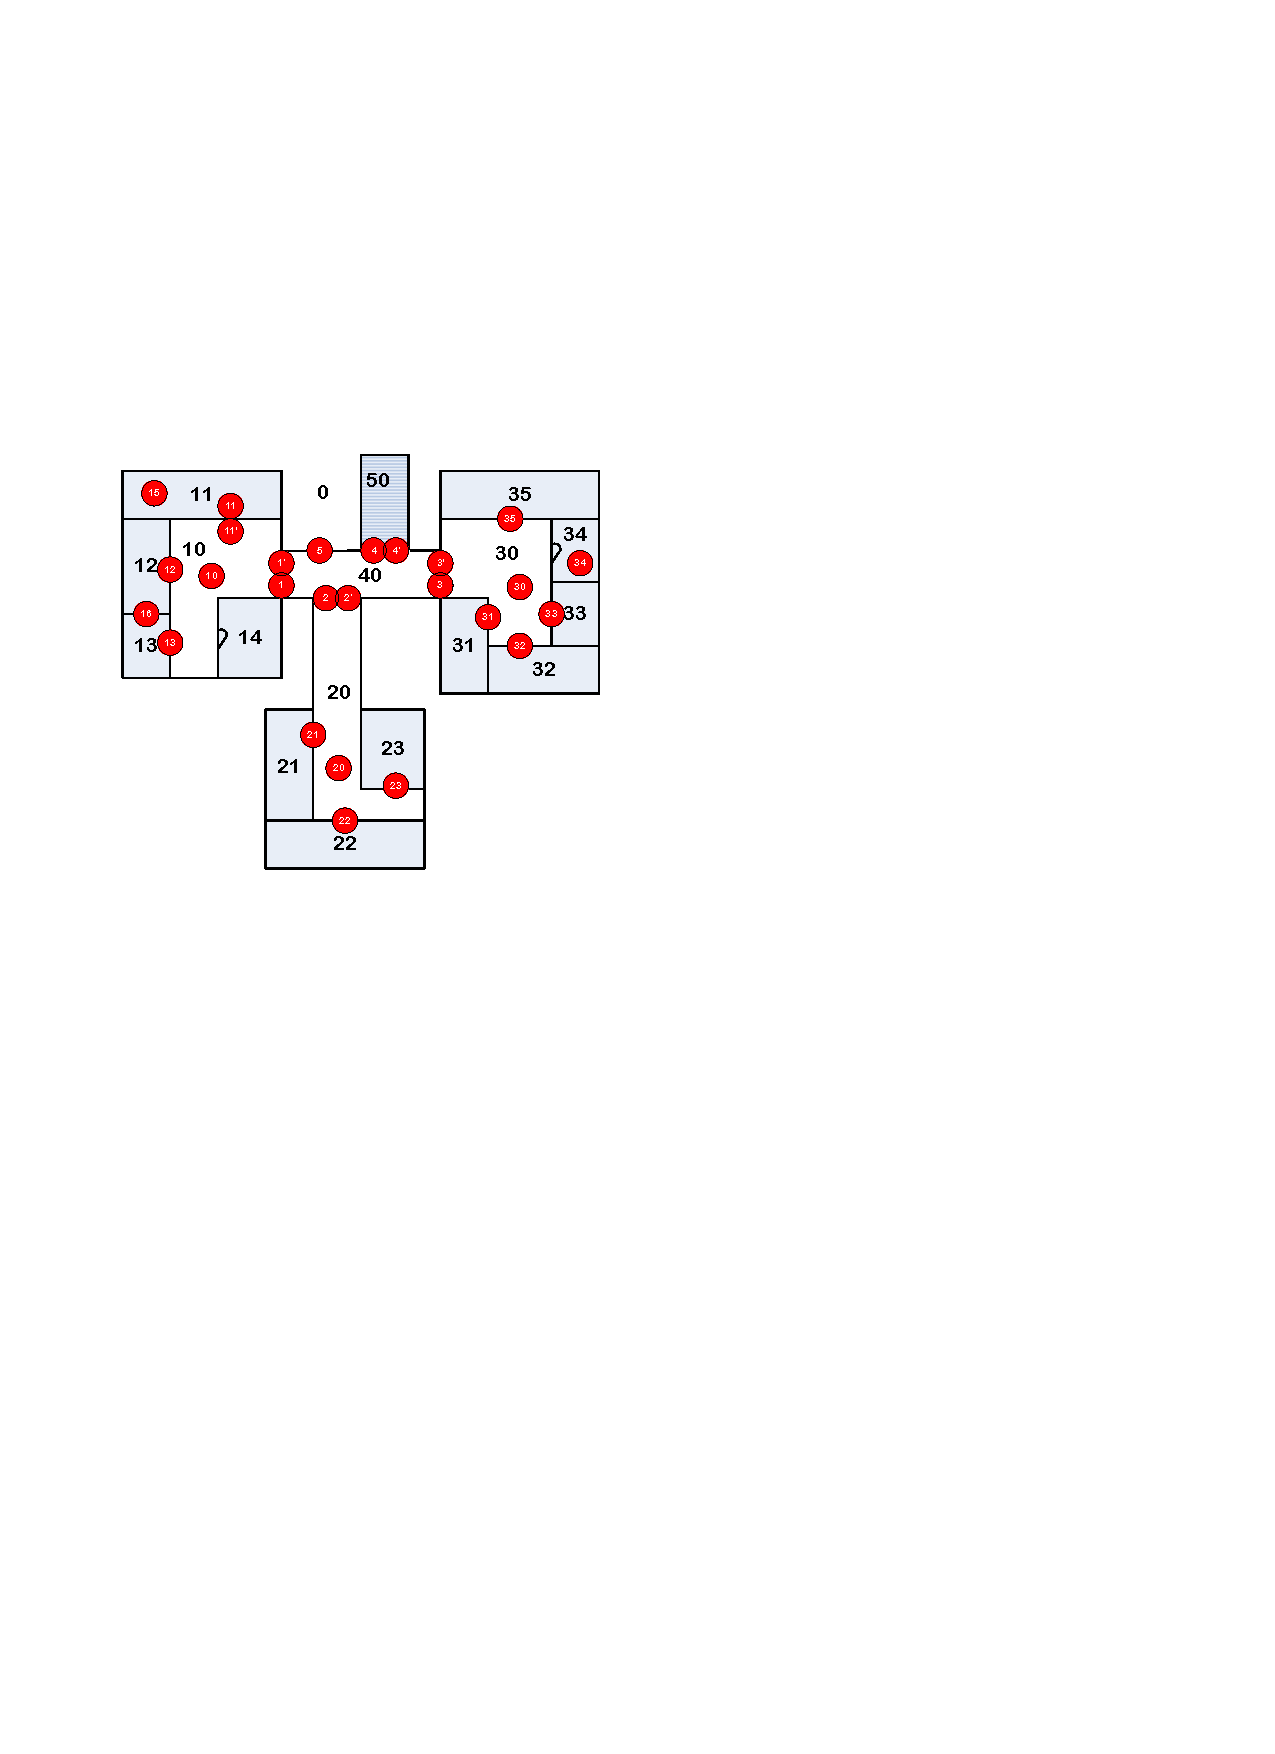
\includegraphics[width=\columnwidth]{figures/2-2/2-2-1.pdf}
    \end{figure}
    \vspace{-20pt}
    \pause
    \begin{figure}[tb]
      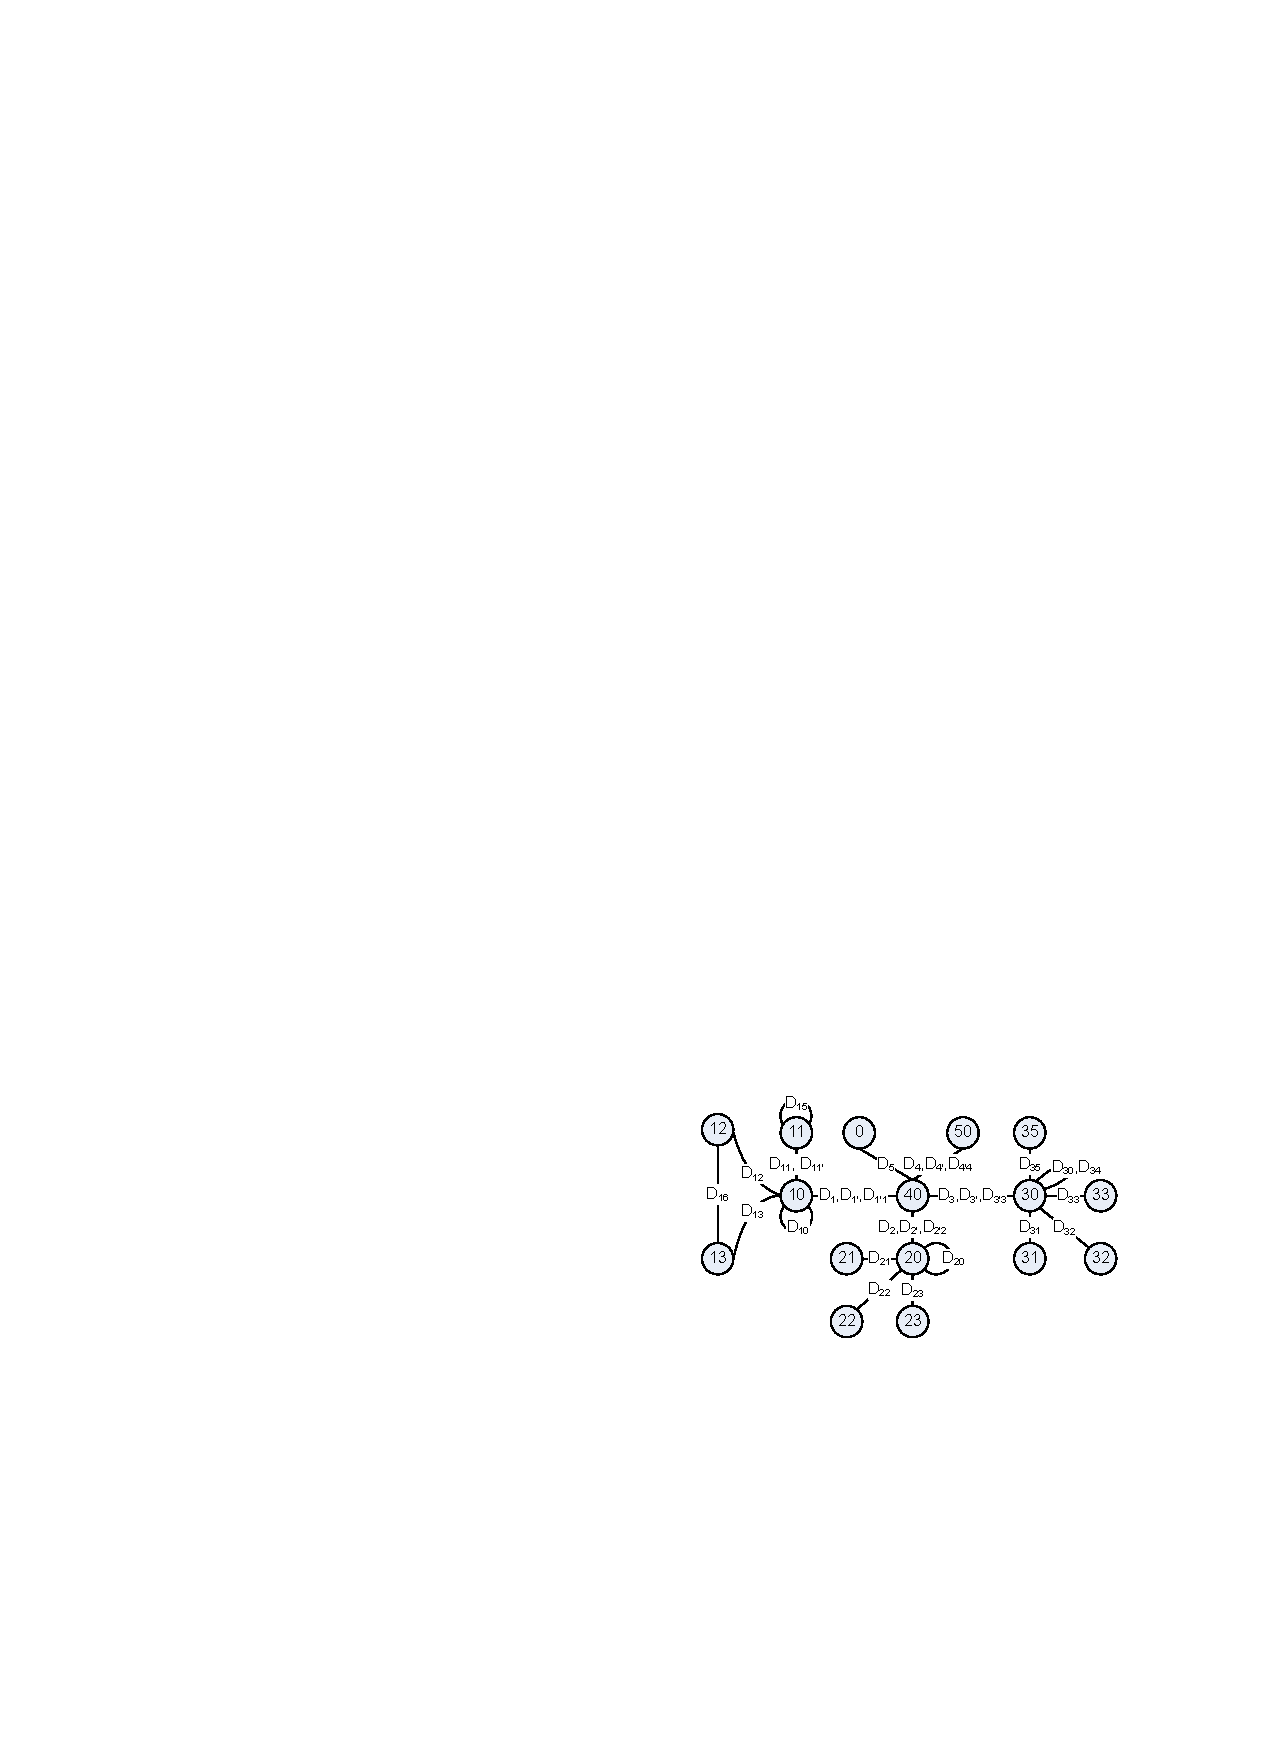
\includegraphics[width=\columnwidth]{figures/2-2/2-2-2.pdf}
    \end{figure}

\end{columns}

\end{frame}

%------------------------------------------------

\begin{frame}
\frametitle{States of Indoor Moving Objects}

%\begin{columns}[c]

  %\column{.57\textwidth}
  \begin{figure}[tb]
    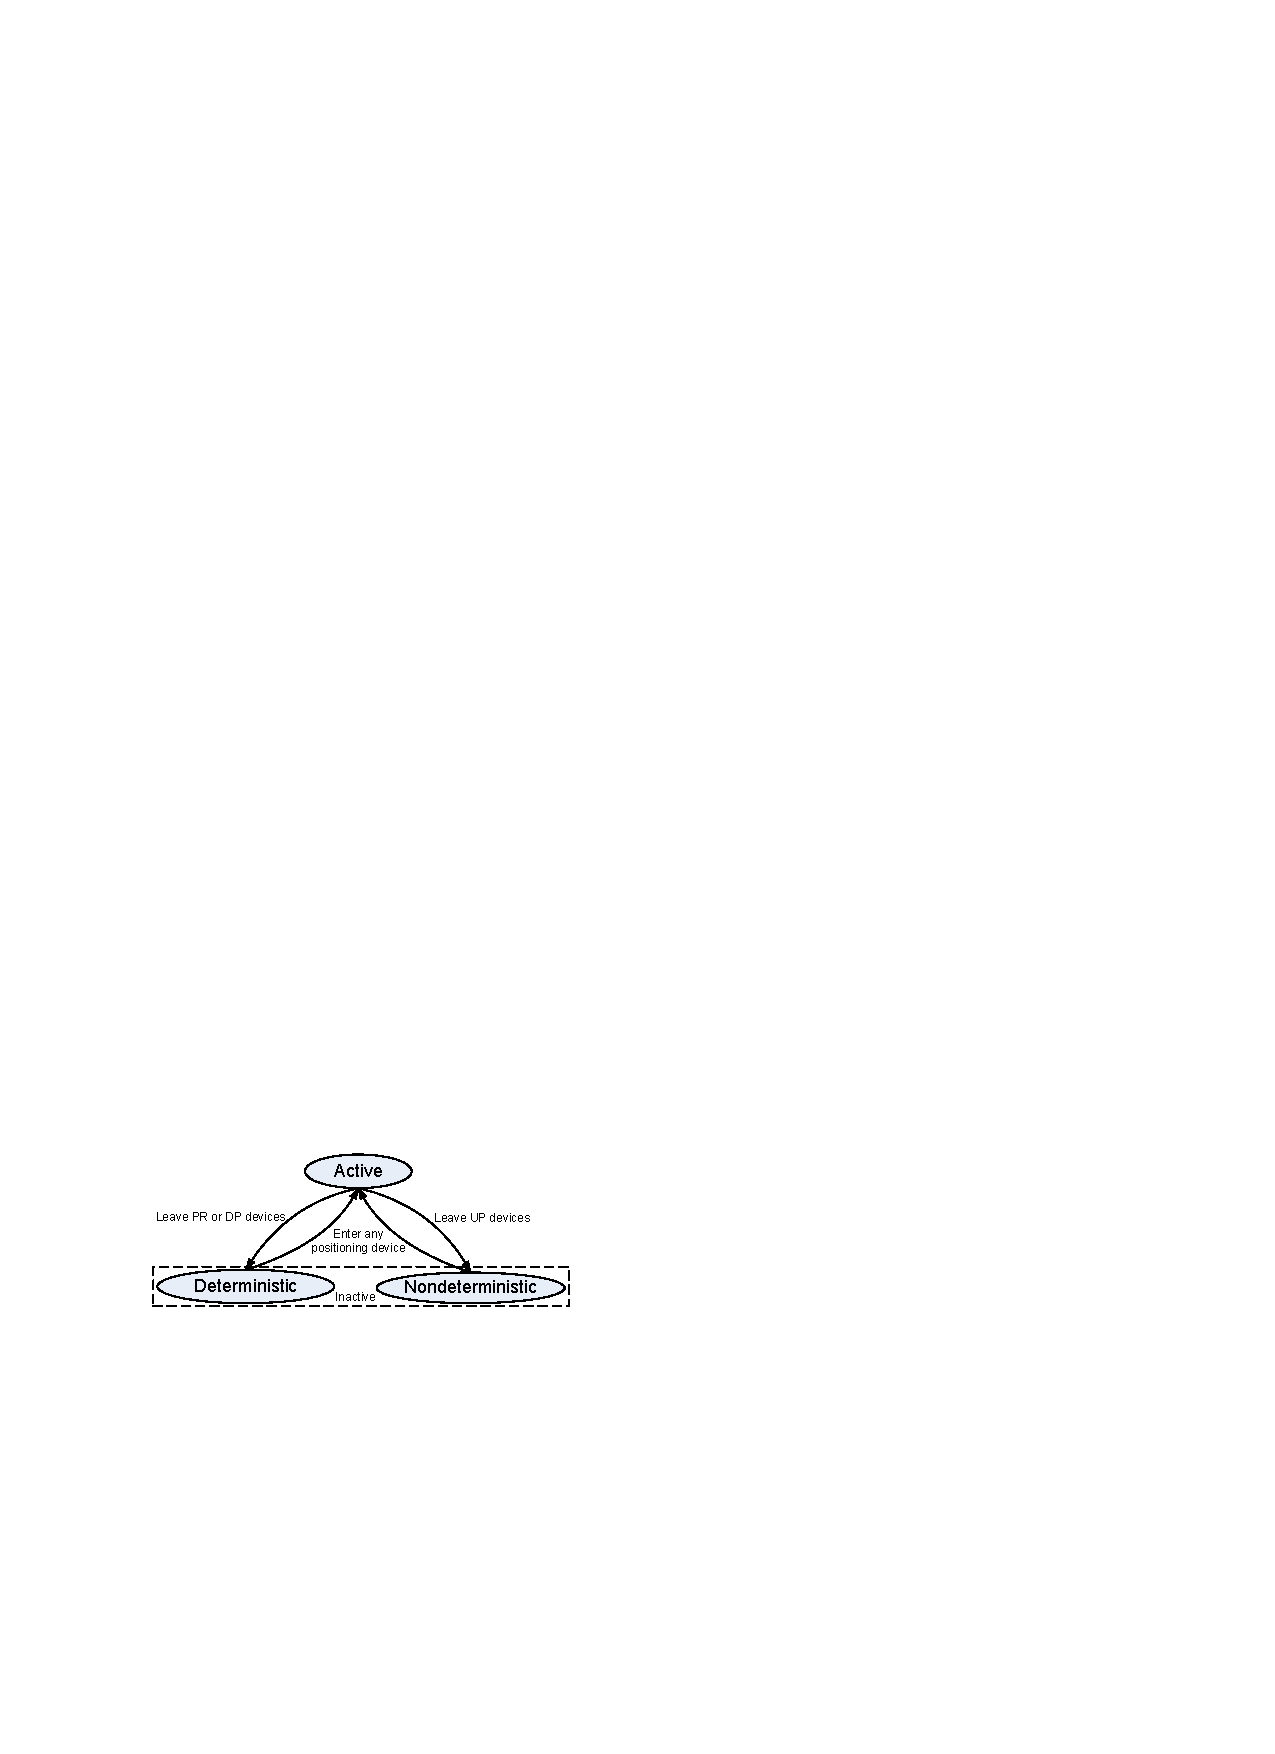
\includegraphics[width=0.6\columnwidth]{figures/2-2/2-2-3.pdf}
  \end{figure}
  \vspace{-10pt}
  %\column{.43\textwidth}
  \begin{itemize}
    \item An object is in an \textbf{active state} when it is inside the activation range of a positioning device.
    \item Otherwise the object is in an \textbf{inactive state}
    \item When an object is in the inactive state it is
      \begin{itemize}
        \item \textbf{nondeterministic} if it can be in more than one cell
        \item \textbf{deterministic} if it is in one specific cell
      \end{itemize}
  \end{itemize}

%\end{columns}

\end{frame}

%------------------------------------------------

\begin{frame}
\frametitle{Indexing Indoor Moving Objects}

\textbf{The proposed indexing scheme uses 4 hash tables}
\\~\\
\pause

\footnotesize{
\emph{Device Hash Table(DHT)} maps each device to a set of active objects:
\pause
$$\mathnormal{DHT[deviceID] = O_A;~deviceID \in \Sigma_{devices}, O_A \subseteq O_{indoor}}$$
\\~\\
\pause

\emph{Cell Deterministic Hash Table(CDHT)} maps each cell to a set of deterministic objects:
\pause
$$\mathnormal{CDHT[cellID] = O_D;~cellID \in C, O_D \subseteq O_{indoor}}$$
\\~\\
\pause

\emph{Cell Nondeterministic Hash Table(CNHT)} maps each cell to a set of nondeterministic objects:
\pause
$$\mathnormal{CNHT[cellID] = O_N;~cellID \in C, O_N \subseteq O_{indoor}}$$
\\~\\
\pause

\emph{Object Hash Table(OHT)} maps objects to their current data(state, time, cell(s) the object can be in)
\pause
$$\mathnormal{OHT[objectID] = (STATE, t, IDSet);~objectID \in O_{indoor}}$$
\\~\\
\pause
}

\end{frame}

%------------------------------------------------

\begin{frame}
\frametitle{RFID Deployment Graph Construction}

\begin{columns}[c]

  \column{.47\textwidth}
    \begin{figure}[tb]
      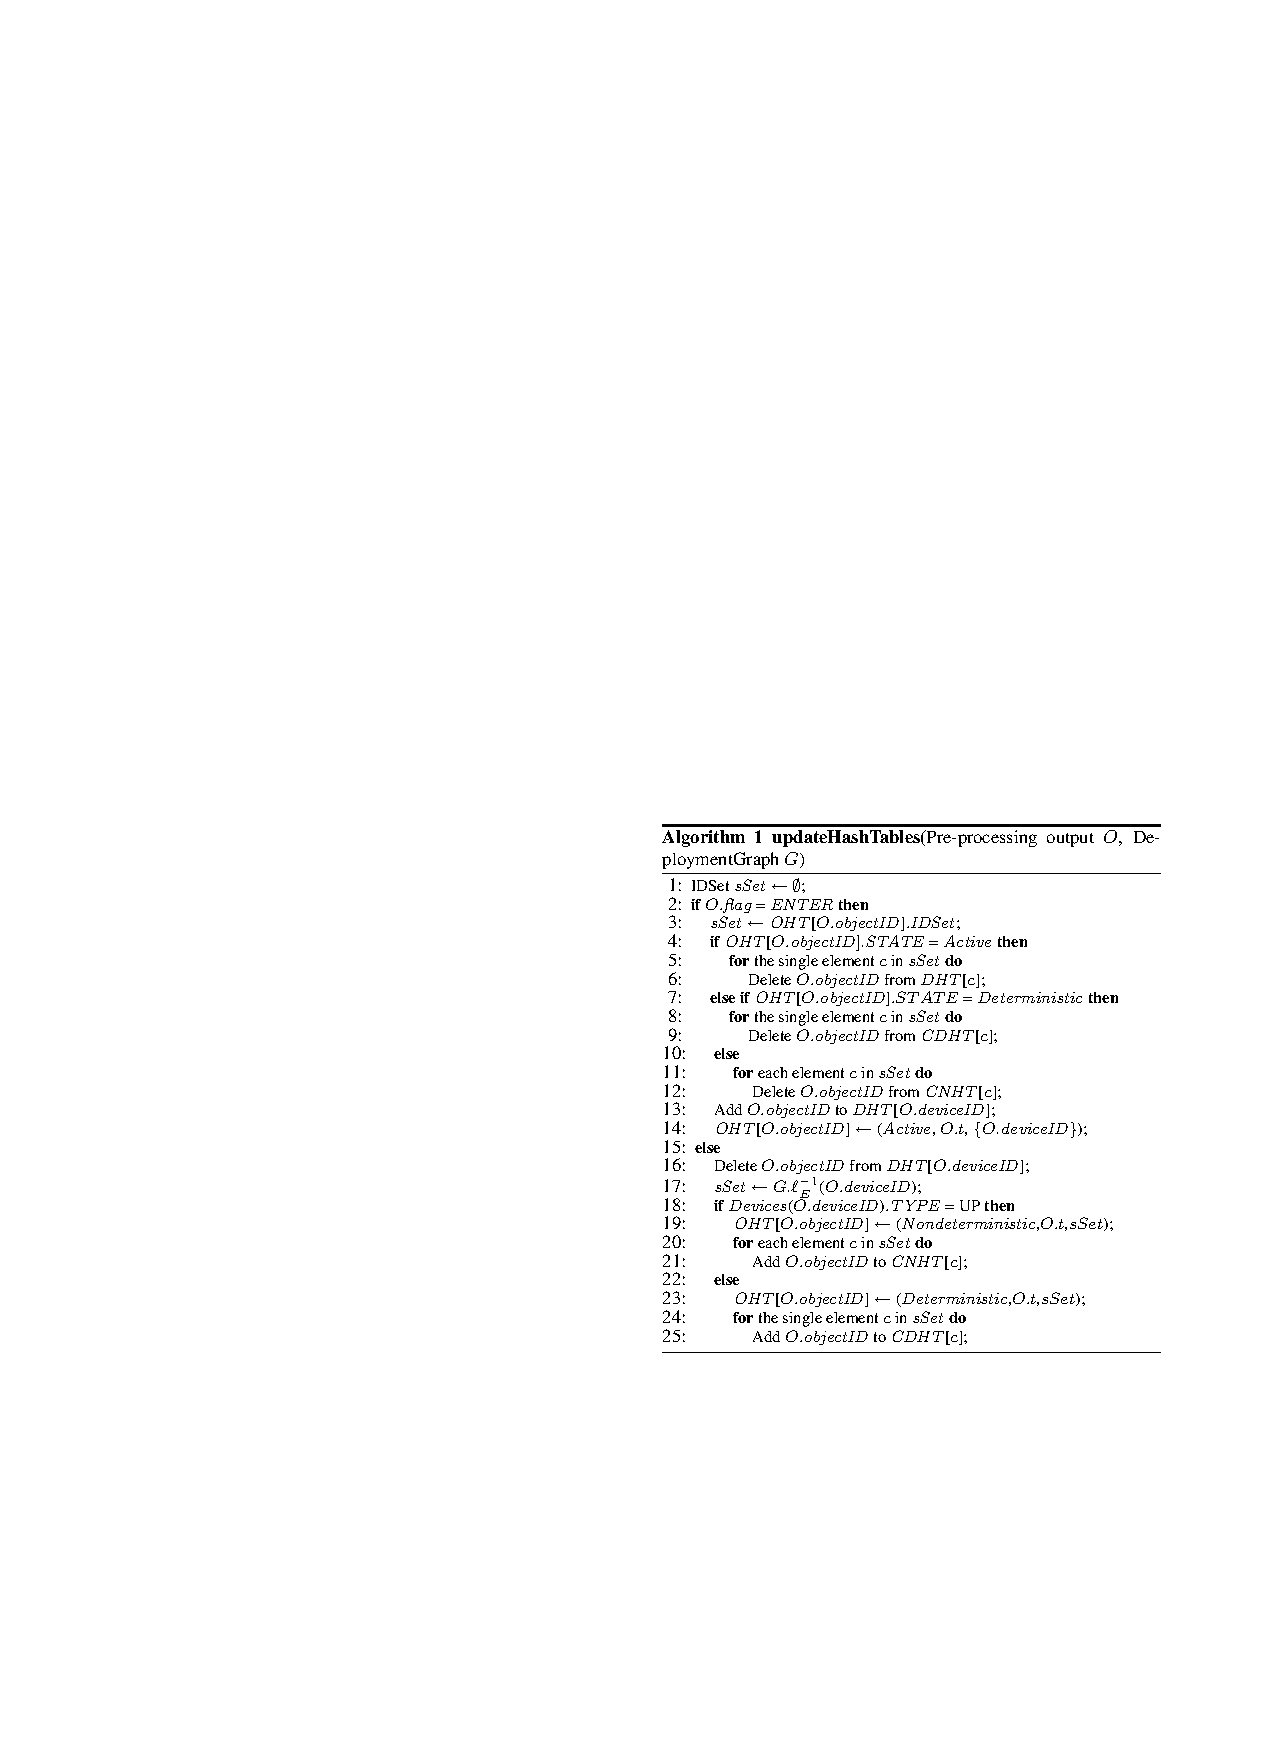
\includegraphics[width=\columnwidth]{figures/2-2/2-2-4.pdf}
    \end{figure}

  \column{.53\textwidth}
  \scriptsize{
    \begin{enumerate}
      \item Lines 1: \textrm{reset $\mathnormal{IDSet}$} \pause
      \item Lines 2--12: \textrm{$\mathnormal{O.flag}$ is ENTER so check the object's previous state. Remove $\mathnormal{O}$ from the corresponding table according its previous state} \pause
      \item Lines 13--14: \textrm{add $\mathnormal{O}$ to table of active objects (DHT), and update $\mathnormal{O}$'s in the objects' table (OHT)} \pause
      \item Lines 16--17: \textrm{$\mathnormal{O.flag}$ is LEAVE so remove the object from DHT. Get the possible cells that $\mathnormal{O}$ can move to} \pause
      \item Lines 18--25: \textrm{if the device is undirected, set $\mathnormal{O}$ in OHT and add $\mathnormal{O}$ to CNHT for the cells in sSet, else apply the same to CDHT}
    \end{enumerate}
  }
  \end{columns}

\end{frame}

%------------------------------------------------

\begin{frame}
\frametitle{Continuous Range Monitoring: Query Definition}

\begin{itemize}
  \item A \emph{Continuous Range Monitoring Query} (CRMQ)
    \begin{itemize}
      \item takes an \textbf{indoor spatial range} $\bf \mathnormal{R}$ as parameter
      \item keeps reporting the objects when it is registered for a certain time frame $\mathnormal{[t_s, t_e]}$
    \end{itemize}
  \item The \textbf{query result} $\bf \mathcal{M}$ -- the set of moving objects in $\bf \mathnormal{R}$ - is maintained as follows:
    \begin{equation*}
      \mathnormal{
      \forall t \in [t_s, t_e]: o \in CRMQ[R](\mathcal{M})  \Leftrightarrow o \in \mathcal{M} \wedge pos_{\mathcal{M}}(o, t) \in R
      }
    \end{equation*}
    where $\mathnormal{pos_\mathcal{M}}$ is a function that can determine the position of object $\mathnormal{o}$ at time $\mathnormal{t}$
  \item Multiple monitoring queries may coexist
\end{itemize}

\end{frame}

%------------------------------------------------

\begin{frame}
\frametitle{Critical Devices}

For a \textrm{CRMQ} query, a \emph{critical device} is one from which a new observation can potentially change the query result (either certain or uncertain)
\begin{columns}[c]

  \column{.4\textwidth}
    \begin{figure}[tb]
      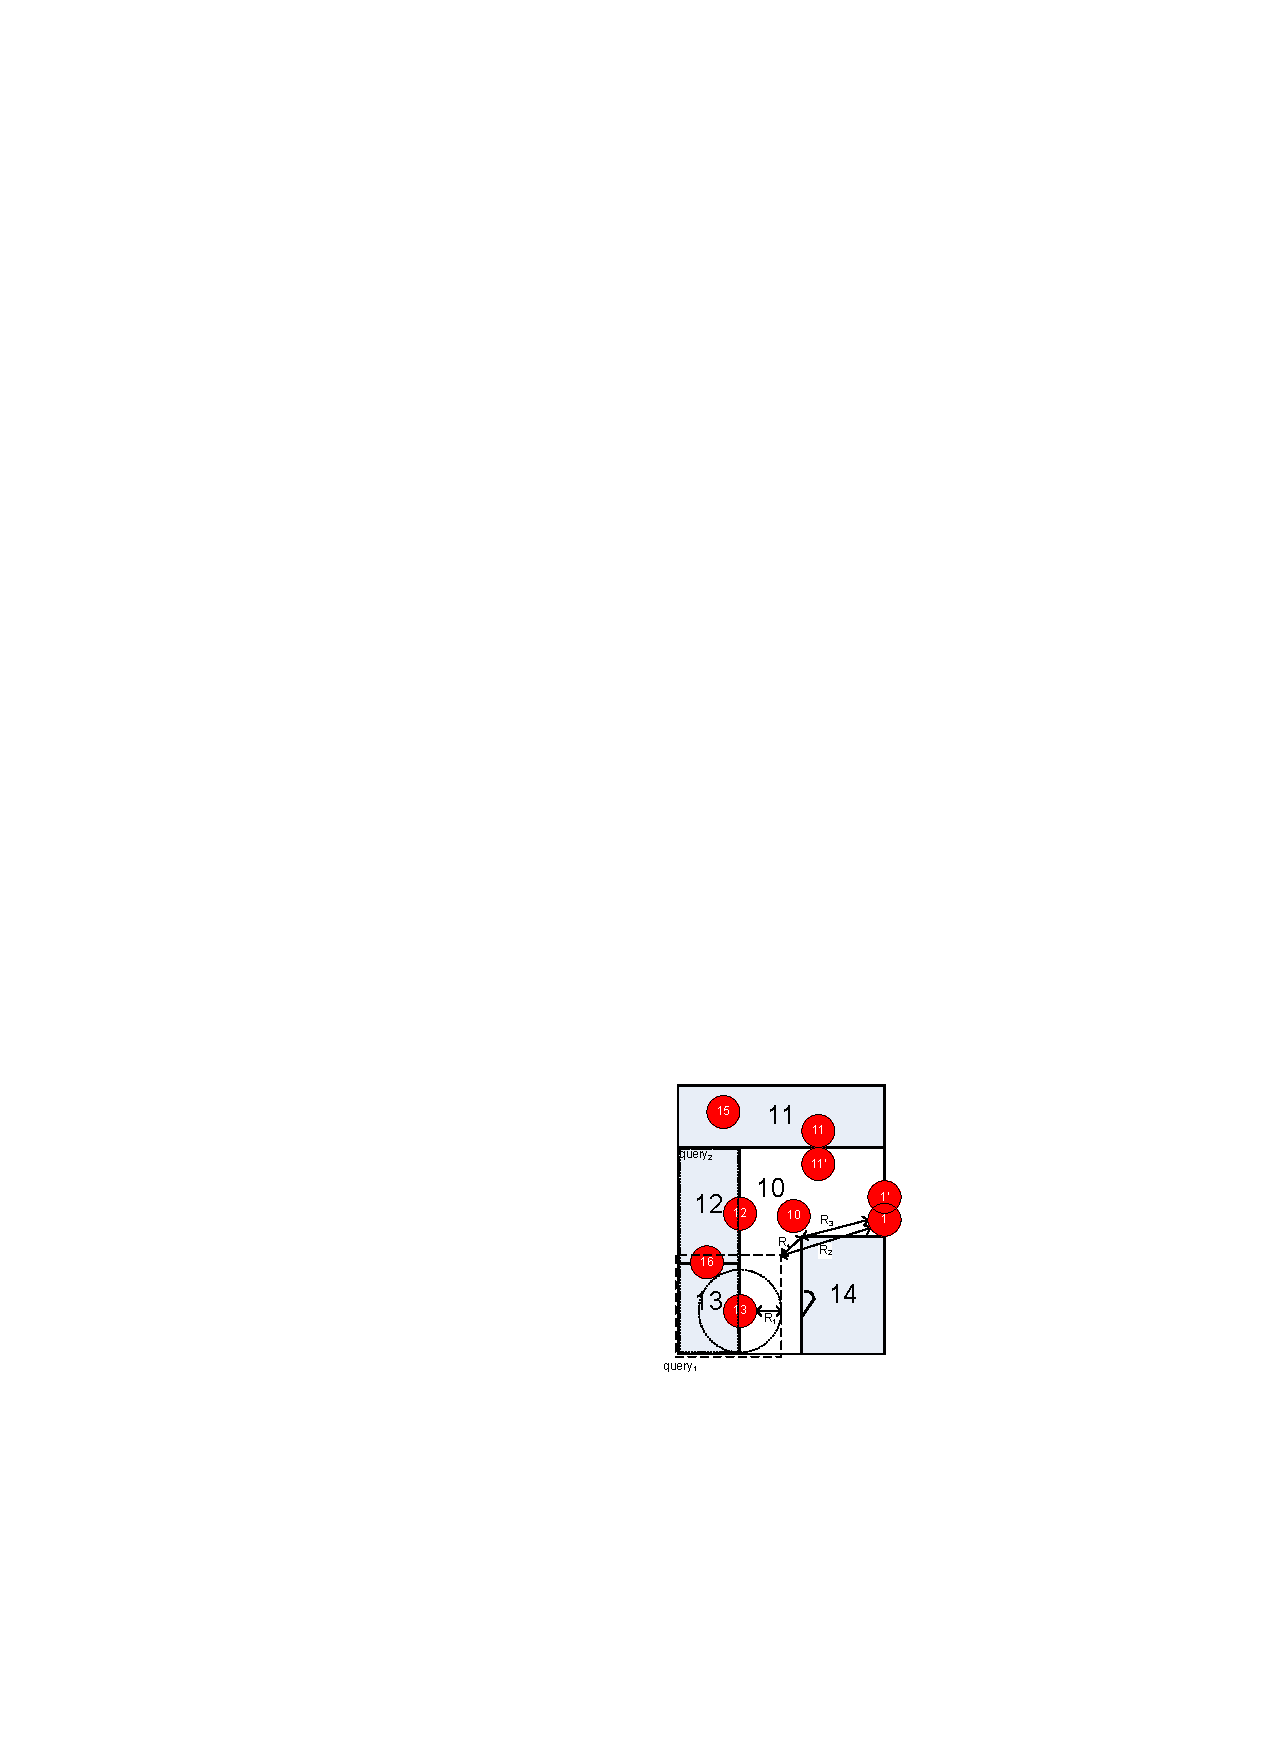
\includegraphics[width=\columnwidth]{figures/2-2/2-2-5.pdf}
    \end{figure}

  \column{.6\textwidth}
    \vspace{-20pt}
    \begin{itemize}
      \scriptsize{
      \item $\mathrm{CLASS1}$ -- \textrm{Device is fully covered in $\mathnormal{R}$ along with cells, e.g., $\mathnormal{(device_{16}, query_2)}$}
      \item $\mathrm{CLASS2}$ -- \textrm{Device is fully covered but corresponding cells are not,  e.g., $\mathnormal{(device_{13}, query_1)}$}
      \item $\mathrm{CLASS3}$ -- \textrm{Device intersects with the query range $\mathnormal{R}$,  e.g., $\mathnormal{(device_{16}, query_1)}$}
      \item $\mathrm{CLASS4}$ -- \textrm{Device is disjoint from $\mathnormal{R}$ and at least one of its corresponding cells in $\mathnormal{C_{ic} = \{ c|c \sqcap R \neq \varnothing \}}$,  e.g., $\mathnormal{(device_{1}, query_1)}$}
      \item $\mathrm{CLASS5}$ -- \textrm{Device is disjoint from $\mathnormal{R}$ and at least one of its corresponding cells in $\mathnormal{C_{ex} = \{ c| \{ c, c'\} \in G.E, c' \in C_{ic} \}}$, but none of them are in $\mathnormal{C_{ic}}$, e.g., $\mathnormal{(device_{10}, query_2)}$}
      }
    \end{itemize}

\end{columns}

\end{frame}

%------------------------------------------------

\begin{frame}
\frametitle{Critical Devices}

\begin{itemize}
  \item To handle concurrent \textrm{CRMQ}s, a \emph{Query Hash Table} is created hold the results
    \begin{itemize}
      \item $\mathnormal{QHT[queryID] = (CR, UR);~ CR \subseteq O_{indoor}, UR \subseteq O_{indoor}}$
      \item where $\mathnormal{CR}$ is the certain result and $\mathnormal{UR}$ is the uncertain result
    \end{itemize}
  \item Overview
    \begin{figure}[tb]
      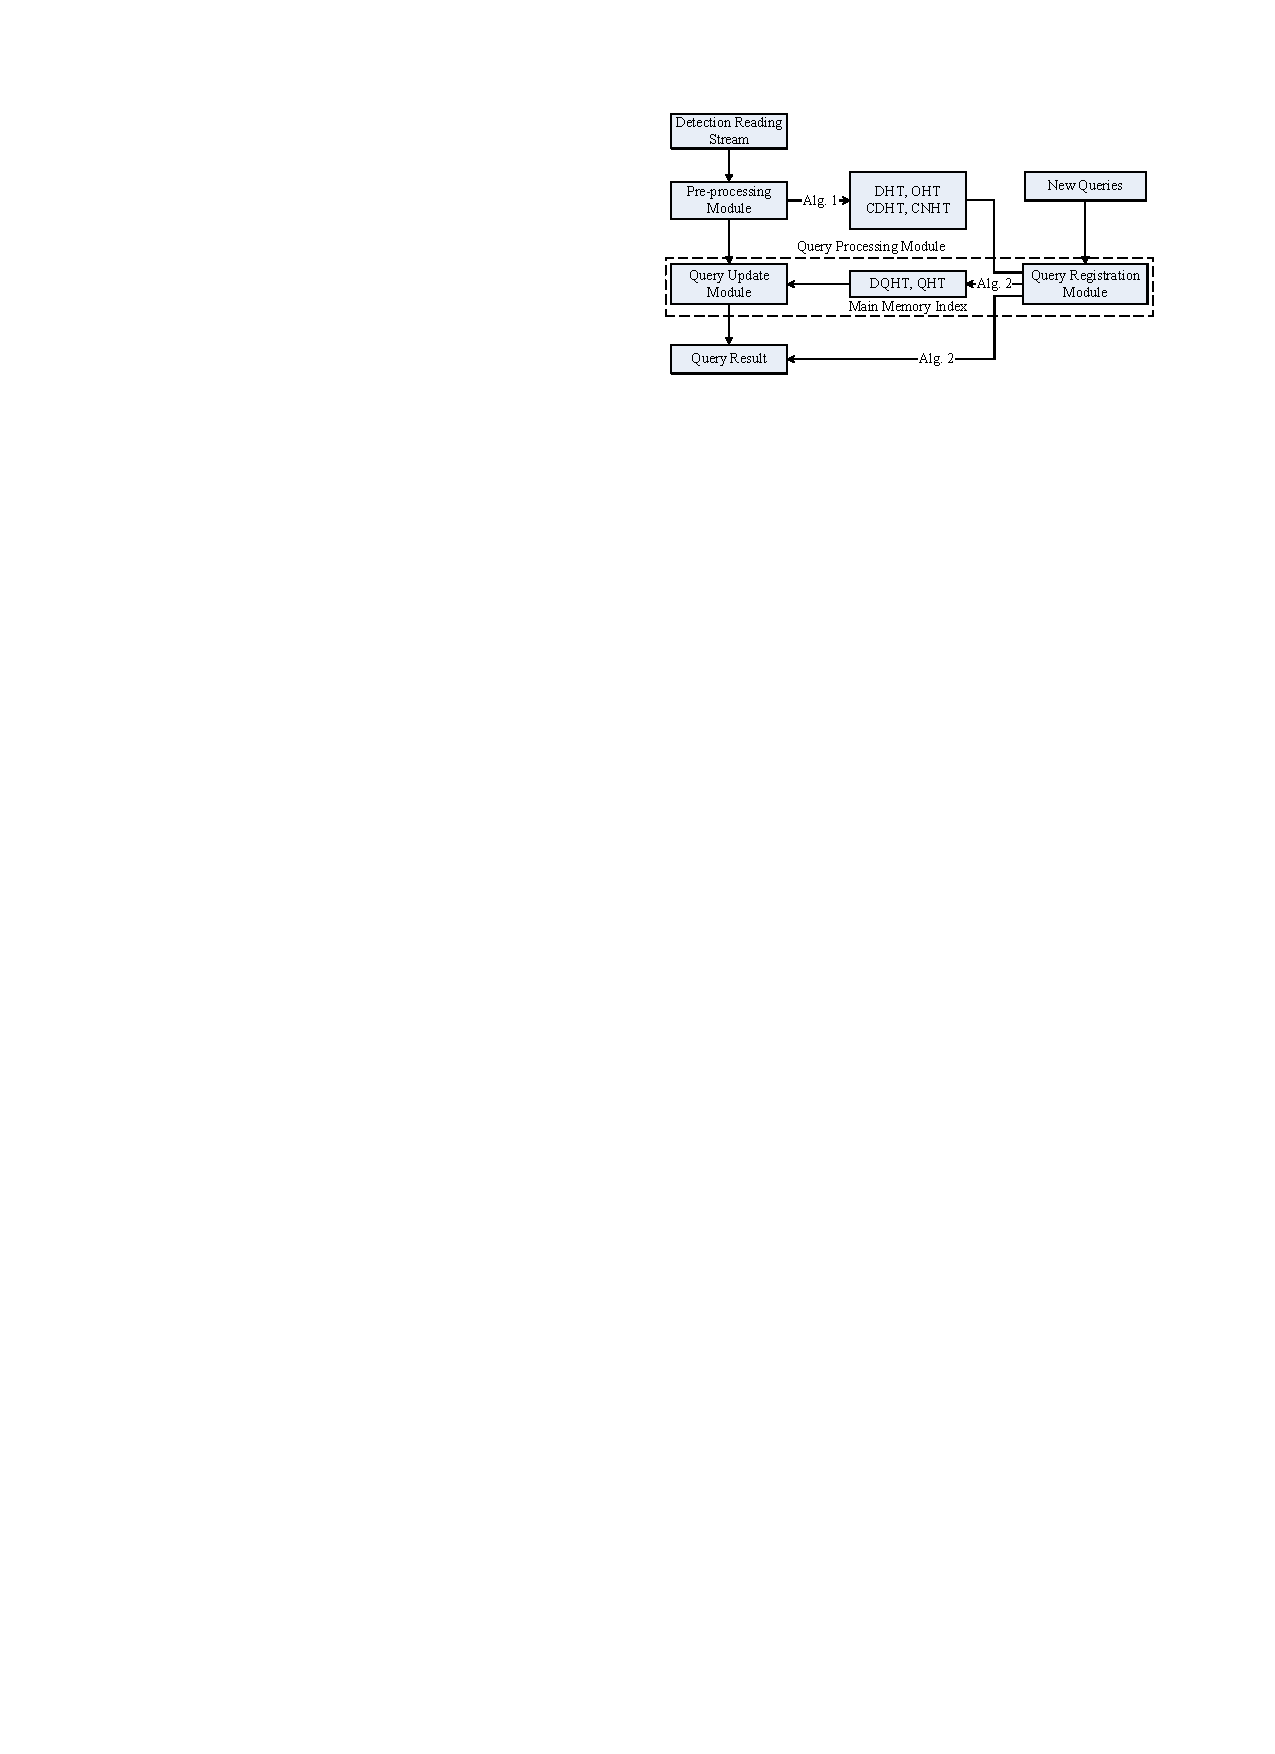
\includegraphics[width=0.68\columnwidth]{figures/2-2/2-2-6.pdf}
    \end{figure}
\end{itemize}

\end{frame}
